\documentclass[11 pt]{article}
\usepackage{amsmath, amssymb, color, xcolor}
\usepackage{graphicx, wrapfig, float, caption, dsfont}
\usepackage{fullpage}
\usepackage[backref=page, hidelinks, colorlinks=true, citecolor=blue!60!black!100]{hyperref}
\usepackage{tikz}
\usetikzlibrary{arrows.meta, shapes}
\usepackage{caption, subcaption}
\usepackage{natbib} % gives us \citet: Author (year) and \citep: (Author; year)
\usepackage{authblk}

\newcommand{\plr}[1]{{\color{blue}\it #1}}
\newcommand{\jss}[1]{{\color{olive}\it #1}}
% \newcommand{\ddt}{\frac{d}{dt}}
\newcommand{\ddt}{\dot}
\newcommand{\ro}{{ro}}
\newcommand{\nro}{{\bar{r}o}}
\newcommand{\rno}{{r\bar{o}}}
\newcommand{\nrno}{{\bar{r}\bar{o}}}
\newcommand{\reachable}{\mathcal{R}}
\newcommand{\unobservable}{\bar{\mathcal{O}}}
\newcommand{\R}{\mathbb{R}}
\newcommand{\E}{\mathbb{E}}
\renewcommand{\P}{\mathbb{P}}
\newcommand{\pda}{\frac{\partial}{\partial A_{ij}}}
\newcommand{\ind}{\mathds{1}}

\DeclareMathOperator{\spn}{span}

\newtheorem{theorem}{Theorem}
\newtheorem{lemma}{Lemma}
\newtheorem{definition}{Definition}
\newtheorem{example}{Example}

\begin{document}

  \section{\emph{S. cerevisiae} galactose catabolism network}

  Yeast galactose catabolism is accomplished via a complex system of molecules including enzymes, transporters, and transcription factors. The GAL2 gene encodes a transporter than imports galactose into the cell cytoplasm. GAL1, GAL7, and GAL10 encode components of enzymes that act sequentially to metabolize the imported galactose. Furthermore, in \emph{S. cerevisiae} the enzyme encoding genes, GAL1, GAL7, and GAL10 are encoded within the same regulon (on the same chromosome and regulated by the same promoter), whereas GAL2 is encoded on a separate chromosome. The transcription factor produced by GAL4 binds to promoter of the regulon, inducing the expression of the enzymes. Another gene, MIG1, which is induced by the presence of glucose, encodes a repressor for the GAL regulon. MIG1 acts by repressing the GAL enzymes, as well as down regulating some of the GAL transcription factors, by repressing GAL4 and GAL3, but not acting on GAL80. MIG1 also represses the transporter GAL2.

   \begin{figure}
        \begin{center}
            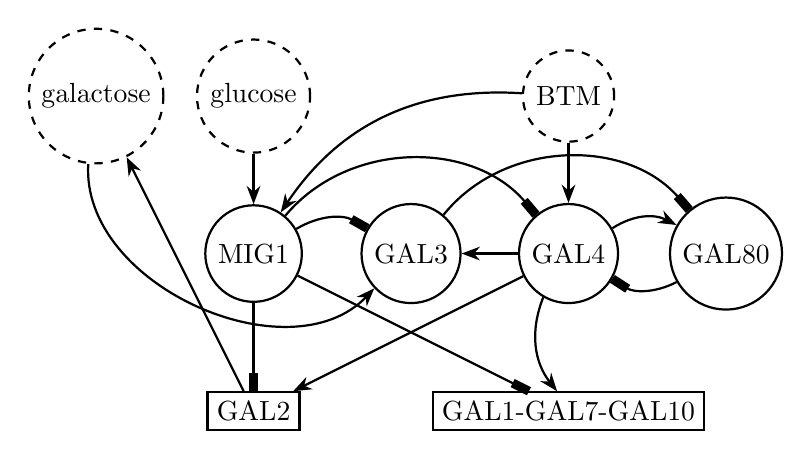
\begin{tikzpicture}
            \begin{scope}[every node/.style={circle,thick,draw}]
                \node (GAL3) at (2,0) {GAL3};
                \node (GAL4) at (4,0) {GAL4};
                \node[dashed] (BTM) at (4,2) {BTM};
                \node (GAL80) at (6,0) {GAL80};
                \node (MIG1) at (0,0) {MIG1};
                \node[shape=rectangle] (GAL2) at (0,-2) {GAL2};
                \node[shape=rectangle] (enzymes) at (4,-2) {GAL1-GAL7-GAL10};
                \node[dashed] (galactose) at (-2, 2) {galactose};
                \node[dashed] (glucose) at (0,2) {glucose};
            \end{scope}

            \begin{scope}[>={Stealth[black]},
                          every edge/.style={draw=black, thick}]
                 \path[->] (GAL4) edge[left] node {} (GAL3);
                 \path[->] (GAL4) edge[bend left] node {} (GAL80);
                 \path[->, >=Rectangle] (GAL3) edge[bend left=50] node {} (GAL80);
                 \path[->, >=Rectangle] (GAL80) edge[bend left] node {} (GAL4);
                 \path[->] (GAL4) edge[bend right] node {} (enzymes);
                 \path[->] (GAL4) edge[left] node {} (GAL2);
                 \path[->, >=Rectangle] (MIG1) edge[bend left] node {} (GAL3);
                 \path[->, >=Rectangle] (MIG1) edge[bend left=50] node {} (GAL4);
                 \path[->, >=Rectangle] (MIG1) edge node {} (enzymes);
                 \path[->, >=Rectangle] (MIG1) edge node {} (GAL2);
                 \path[->] (glucose) edge node {} (MIG1);
                 \path[->] (galactose) edge[bend right=70] node {} (GAL3);
                 \path[->] (GAL2) edge node {} (galactose);
                 \path[->] (BTM) edge node {} (GAL4);
                 \path[->] (BTM) edge[bend right] node {} (MIG1);
            \end{scope}
            \end{tikzpicture}
        \end{center}
        \caption{
          Yeast galactose catabolism transcription network.}
    \end{figure}

    \begin{align*}
      \dot{x}(t) &= \begin{bmatrix} 0 & + & 0 & - \\ 0 & 0 & - & - \\ - & + & 0 & 0 \\ 0 & 0 & 0 & 0 \end{bmatrix} \begin{bmatrix} \text{GAL3} \\ \text{GAL4} \\ \text{GAL80} \\ \text{MIG1} \end{bmatrix}(t) + \begin{bmatrix} + & 0 & 0 \\ 0 & 0 & + \\ 0 & 0 & 0 \\ 0 & + & + \end{bmatrix} \begin{bmatrix} \text{galactose} \\ \text{glucose} \\ \text{BTM} \end{bmatrix}(t) \\
        y(t) &= \begin{bmatrix} 0 & + & 0 & - \end{bmatrix} \vec{x}(t)
    \end{align*}

    In the above parameterization, $y(t)$, or the cumulative impact of transcriptional regulation on the expression of the GAL regulon, will either tend towards positive or negative infinity depending on the ratio of galactose to glucose, and the impact of the basal transcriptional machinery (BTM) on the components of the system.
    \subsection{concrete example}
    \begin{align*}
      \dot{x}(t) &= \begin{bmatrix} 0 & 1 & 0 & -1 \\ 0 & 0 & -1 & -1 \\ -1 & 1 & 0 & 0 \\ 0 & 0 & 0 & 0 \end{bmatrix} \begin{bmatrix} \text{GAL3} \\ \text{GAL4} \\ \text{GAL80} \\ \text{MIG1} \end{bmatrix}(t) + \begin{bmatrix} 1 & 0 & 0 \\ 0 & 0 & 1 \\ 0 & 0 & 0 \\ 0 & 1 & 1 \end{bmatrix} \begin{bmatrix} \text{galactose} \\ \text{glucose} \\ \text{BTM} \end{bmatrix}(t) \\
        y(t) &= \begin{bmatrix} 0 & 1 & 0 & -1 \end{bmatrix} \vec{x}(t)
    \end{align*}
    \begin{align*}
      H(z) = \begin{bmatrix} 1 \\ z^{2} + z + 1 \\ z + 1 \end{bmatrix} \frac{1}{z^{3} + z -1}
    \end{align*}

    \begin{align*}
      CV &= C \\
      VB &= B \\
      V :&= \begin{bmatrix} 1 & 0 & a & 0 \\ 0 & 1 & 0 & 0 \\ 0 & 0 & b & 0 \\ 0 & 0 & 0 & 1 \end{bmatrix} , V^{-1} = \begin{bmatrix} 1 & 0 & \frac{-a}{b} & 0 \\ 0 & 1 & 0 & 0 \\ 0 & 0 & \frac{1}{b} & 0 \\ 0 & 0 & 0 & 1\end{bmatrix} \\
        A(a,b) :&= VAV^{-1} = \begin{bmatrix} -a & a+1 & \frac{a^{2}}{b} & -1 \\ 0 & 0 & \frac{-1}{b} & -1 \\ -b & b & a & 0 \\ 0 & 0 & 0 & 0 \end{bmatrix}
    \end{align*}
    The GAL regulatory network in \emph{S. cerevisiae} is modelled here. The activating transcription factor GAL4, which is regulated by the presence of galactose and two other TFs, binds to the promoter region of the GAL regulon -- a cluster of genes regulated by the same promoter encoding 3 enzymes (GAL1, GAL7, and GAL10), for the metabolism of the sugar galactose. The repressing transcription factor MIG1, which is activated by the presence of glucose and other proteins omitted here, also binds to the regulon, preventing the expression of the galactose metabolizing enzymes. This network is one of the most studied gene regulatory networks in yeast, and experiments have already demonstrated significant transcriptional variation among different species and genuses of yeast.

    In the present model, the $A$ matrix encodes the interactions among GAL3, GAL4, GAL80, and MIG1. $B$ interprets the input: the quantity of glucose, galactose, and the basal transcription (BTM) rates impact of TF concentrations. $C$ represents the promoter region of the GAL regulon and is the sum of the influence of GAL4 (activating) and MIG1 (repressing).

    $A(a,b)$ represent alternative network structures that produce identical outputs, with identical input and output transformations -- meaning the regulatory contributions of the sugars and the basasl machinery, as well as the promoter of the GAL regulon are held constant. These interactions may be realized in nature, if the regulatory differences predicted by $A(a,b)$ are biologically/mutationally realizable. Mutations influencing the interactions between GAL4 and GAL80 have been experimentally demonstrated \citep{li2010alterations}.

    Furthermore, our fitness function is restricting the network to realize the transfer function $H(z)$ exactly. We see this as justifiable, as experiment has shown the output of a metabolic regulatory network directly influences organismal growth rates. In \citet{dekel2005optimality} \emph{E. coli} that over or under express lactase, governed by the \emph{lac} operon, in a given sugar environment, their fitness (growth rate) suffers.

    We are interested in network rewiring rates. This can be modelled as a Brownian motion of the free parameters,
    \begin{align*}
      A_{t} &= A(f(W_{t}), g(W_{t})) \\
      \mathbb{E} [ | A_{\epsilon} - A_{0} | ] &= \epsilon + \mathcal{O}(\epsilon^{2})
    \end{align*}

    This realization is minimal as the rank of both the reachability and observability matrices is full ($4$).

    Note: check that $V$ is the \emph{only} invertible matrix that preserves $C$ and $B$. 
    \subsection{Notes}
    \begin{itemize}
      \item The interaction strength between GAL4 and GAL80 can be altered via mutation. Furthermore, a mutation in GAL4 that decreases affinity can be compensated by a mutation in GAL80 \citep{li2010alterations, salmeron1990gal4, adhikari2014perturbation}.
      \item The galactose metablic network shows tremendous regulatory variation among different species of yeast \citep{lavoie2009rearrangements, martchenko2007transcriptional, dalal2016transcriptional, christensen2011unique, hartl2007induction, alam2013aspergillus}.
      \item GAL3 (a TF) is a paralog of GAL1 (enzyme), yet GAL3 no longer has any galactokinase activity. GAL1, however, can weakly regulate in place of GAL3.
      \item RTG1-RTG3 regulates the Gal regulon in other species of yeast. 
    \end{itemize}

    \section{Cell Cycle Control}
      The cell cycle, and the initiation of cellular processes in general, is often triggered by the simultaneous presence and absence of specific molecules. In yeast, traversal through the cell cycle is largely determined by the presence of a class of proteins called cyclins. Cyclin concentration levels oscillate throughout the cell cycle, and after reaching a threshold interact with CDKs, triggering a transition to another phase of cellular life. Although the underlying mechanics controllying cell cycle phase transitions is extremly complex, involving many steps including transcriptional regulation and enzyme phosphorylation, several lines of evidence suggest that the simple oscillating expression patterns of transcription factors is important for cell cycle control \citep{orlando2008global, simon2001serial}. 
      \begin{quote}
        We propose that periodic transcription is an emergent property of a transcription factor network that can function as a cell-cycle oscillator independently of, and in tandem with, the CDK oscillator. \citep{orlando2008global}
      \end{quote}

      \subsection{Notes}
      \begin{itemize}
        \item According to \citet{cross2011evolution}, the network topology and dynamic properties of cell cycle control in both yeast and mammals is highly conserved, however the proteins themselves are highly diverged -- even having completely unrelated amino acid sequences.
        \item Mammalian G1-S regulation is more complex than yeast: the mammalian system contains addition feedback loops. Furthermore, CDKs ``play complementary roles'' as both CDK4 and CDK6 both bind cylicn D and CDK1 and CDK2 both bind to cyclins, A, B and E. The binding is not very specific as there is significant cross-binding among the CDKs and cyclins \citep{cross2011evolution}.
        \item ``Proteins involved in DNA replication are conserved from yeast to mammals, suggesting that the mechanism was established at an early stage of eukaryotic evolution. In spite of this common origin, recent findings have revealed surprising variations in how replication initiation is controlled, implying that a conserved mechanism has not necessarily resulted in regulatory conservation'' \citep{kearsey2003enigmatic}.
        \item Putative DMI may be gene involved in cell cycle control? Researchers identified regions \emph{hms1} and \emph{hms2} -- or hybrid male sterility 1/2 -- in \emph{Mimulus}. These genomic regions contain genes known to be involved in cell cycle control \citep{sweigart2015evidence}.
      \end{itemize}
    \section{Early Development and Pattern Formation in \emph{Drosophila}}
    \begin{itemize}
      \item DSD in gap gene network lead to DMI in \emph{D. melanogaster} and \emph{D. santomea} (see D. Matute work). 
    \end{itemize}
    \section{Carbohydrate metabolic network in \emph{S. cerevisiae}}

    In Flux Balance Analysis, a metabolic reaction at equilibirum is represented as, 
    \begin{align*}
      Sv = 0
    \end{align*}
    Where, $S$ is an $n \times m$ stochiometric matrix and $v$ is a vector of fluxes through the network. Each column of $S$ is a reaction, and each row is a unique compound. Any vector in the nullspace of $S$ can represent fluxes through the network in steady state. Although flux is a function of enzyme activity, expression level, and substrate concentrations, we may be able to model each element of $v$ as simply enzyme expression levels. Thus, the output of a GRN $y$ can be input as the flux vector for the metabolic network. 
      \begin{itemize}
        \item Integration of Flux Balance Metabloism and TRN models (see B Palsson work).
        \item Could the diversity in wine taste profiles partially be a consequence of DSD in the metabolic reaction network? 
      \end{itemize}
    \section{Circadian clock}
      \begin{itemize}
        \item The Intelligent Clock and the Rube Goldberg Clock \citep{sancar2008intelligent}.
      \end{itemize}
    \section{Chemotaxis in prokaryotes}

\bibliographystyle{plainnat}
\bibliography{krefs}

\end{document}

